% !TeX encoding = UTF-8
% !TeX program = pdflatex
% !TeX spellcheck = en-US

\documentclass[11pt]{article}

\usepackage[english]{babel}
\usepackage{graphicx}
\usepackage{listings}
\usepackage{xcolor}   % for \textcolor
\usepackage{tikz,pgfplots}
\usepackage[htt]{hyphenat}
\usepackage{url}

\lstset
{
  language=C,
  numbers=left,
  stepnumber=1,
  breaklines=true,
  basicstyle=\ttfamily,
  keywordstyle=\color{blue}\ttfamily,
  stringstyle=\color{red}\ttfamily,
  commentstyle=\color{green}\ttfamily,
  morecomment=[l][\color{magenta}]{\#}
  columns=fullflexible,
  postbreak=\mbox{\textcolor{red}{$\hookrightarrow$}\space},
  escapeinside={(*@}{@*)},
}
\lstdefinestyle{nonumbers}
{numbers=none}

\title{RopGun \\ Runtime Detection of ROP Payload Executions\\\bigskip\large Data Centers and High Performance Computing\\Sapienza}
\author{Pietro Borrello}
\date{\today}

\begin{document}

\maketitle

\tableofcontents
\newpage

\section{Introduction}
One of the major today's security challenges is how to deal with memory related attacks. To exploit buffer overflow vulnerabilities in presence of the classical defense mechanisms such as Data Execution Prevention (NX), attackers take advantage of code reuse attacks.

Code-reuse attacks are software exploits in which an attacker directs control flow through existing code with a malicious result, by constructing a chain of small code sequences called gadgets that are present in vulnerable program's memory. Exploits that are based on such techniques are called ROP (Return-Oriented Programming) and are increasingly present in advanced attack scenarios.

Since only relying of memory safe languages would ideally ensure bug free programs, but avoid using languages as C and C++ would be impossible, the scientific community has introduced a plethora of possible mitigation to raise the bar in the development of effective attacks. Techniques as code randomization, code rewriting, control flow integrity or software shadow stack (implemented to prevent return address poisoning), are effective, but they all rely on the compiler support, and are often non applicable,  either due to the lack of source code or debugging information, or due to their increased overhead.

In this paper we analyze and implement {\bf RopGun}: a totally different type of ROP mitigation, that only relies on hardware facilities. It is based on inspecting performance hardware counters to notice abnormal behavior that characterizes the execution of a ROP payload.

\section{Related Works}

\subsection{ROP Attacks}
Return-oriented programming (ROP) is an exploiting technique that allows an attacker to induce arbitrary behavior in a vulnerable program without actually injecting any code, but through a chain of redirections in the program memory itself \cite{rop}. The attack scenario is based on a controlled stack frame, where the return address can be overwritten. This is an advanced version of the “return to libc attack” \cite{ret2libc} where multiple pieces of code are called in sequence to provide the needed code semantics execution: the attack combines a large number of short instruction sequences followed by a {\tt ret} (called gadgets from now on) that allow arbitrary computation. This is resilient to mitigations as non executable memory areas.

Each gadget is in the form of a couple of instructions followed by a return. This allows the attacker to place a sequence of gadget addresses on the stack (called ROPChain) from the return address on, that will be executed thanks to the semantics of the ret instruction. Therefore once the first poisoned return address is met by the first ret, the execution of the chain is triggered, and the first gadget is executed. Once it has executed its instructions it will ``return into'' the next gadget placed on the stack, transferring the control flow to it. And the chain will keep executed gadget after gadget, allowing Turing complete computation.

\subsection{Performance Counter Inspection}
The idea of inspecting hardware facilities to identify abnormal control flow transfers that usually appear when a ROP payload is executing was firstly introduced by {\tt kBouncer} \cite{kbouncer}. Citing them:

``To define the “abnormal” control transfers we take a closer look into how ROP code executes. Before
ROP code starts executing, the register that holds the stack pointer is set to the beginning of the ROP
payload. Then, each gadget ends with a return instruction, which advances the stack pointer to the address
of the next gadget and transfers control to it. At runtime, the return instructions of ROP code can be
easily distinguished from the legitimate return instructions of the actual program, which are paired with
call instructions and transfer control to the instruction following the call. Thus, a return instruction that
transfers control to an instruction not preceded by a call is considered abnormal''

kBouncer checks for abnormal control flows at every syscall, inspecting the {\tt Last Branch Recording} to try to find ROP flows.

Another interesting work in the field is {\tt HDROP} \cite{HDROP} which aims to find abnormal control flows transfers due to ROP Payloads, checking for high indirect branch mis-prediction, at each code page fault from the kernel. It leverages the fact that usually hardware predictors fails to predict effectively return instructions in ROP payloads, since the {\tt Return Address Stack} was not populated with the address as no call preceded the return instruction. To have a low overhead on the system {\tt HDROP} checks for high mis-prediction ratio only at page fault, leveraging the fact that ROP Payloads usually spans more than a page. This still gives the chance for an attacker to compose a ROP chain that spans over a single page.

\section{Attacker Model}
We assume a common attacker model where an attacker can read/write the data section and read/execute the code section of a vulnerable program. We assume defenses like ASLR and DEP are in place, and the attacker is able to hijack the program’s control flow by means of a memory corruption vulnerability.


\section{Design Goals}
In this paper we present {\bf RopGun}, a process monitor to mitigate possible ROP attacks, intercepting them while executing. {\bf RopGun} takes the best parts from both {\tt HDROP} and {\tt kBouncer}.

{\bf RopGun} constantly monitors the ratio of mis-predicted returns for a process. We exploit the fact that branch prediction on returns is usually really precise. It is implemented through the use of a Return Address Stack ({\tt RAS}) with {\tt N} entries, usually with {\tt N = 16}, populated at each call and read at each return to predict the address to return to. Emulating the stack, the  {\tt RAS} is usually precise in predicting the next address, limited only by its size, and by the operating system context switches that can corrupt it. Therefore when the mis-predicted return instructions becomes significantly high, there is an high probability of a ROP payload being run.

While we think that inspecting the ratio of mis-predicted returns is the best way to spot a ROP payload executing, we think that such check should be done at every syscall. This leaves the attacker with no or few possibility to evade the mitigation, apart from switching to way more difficult techniques as Jump-Oriented Programming \cite{jop} or Counterfeit Object-Oriented Programming \cite{coop}.

The tool should ideally block ROP payloads before being able to do any damage, therefore blocking them at syscall gate is the best place to avoid untrusted code to interact with the kernel. {\bf RopGun} should also avoid blocking any process that has a possibly higher ratio of mis-prediction but is not under attack. Therefore we should be able to define empirically or at runtime a suitable threshold of {\tt ret} mis-predictions.

\bigskip
We designed the tool to monitor the mis-prediction ratio between every syscall pair of a process: this avoids the few ret mis-predictions in the ROPChain to be unnoticed between all the rets in the executable. Monitoring only the returns between syscall pairs, makes evident when the ratio of mis-predictions increases due to ROP control flow that needs usually just 20-30 gadgets to express a useful semantics. Moreover, while the first syscall called by the ROPChain could be missed if done at the beginning of the chain, it becomes infeasible (or really difficult) to concretely compose a payload with more than one syscall, since all the control flow in between would be mis-predicted and therefore noticed.

We define two working mode for {\bf RopGun}: {\tt Monitor Mode} and {\tt Killer Mode}. The first mode just passively logs mis-prediction ratios between syscall pairs, identifying them. This can be a useful mode for anyone inspecting a process or predictors behavior, to log performances, and to train for the {\tt Killer Mode}. This second mode is actively monitoring the process, in order to identify ROP payloads given a defined threshold of mis-prediction. If a ROP attack is identified, the process is killed before letting him to complete the syscall, successfully blocking the ROPChain.

{\bf RopGun} will be released open source at \path{github.com/pietroborrello/RopGun}, in the hope that it will be useful to researches digging in the same field, since all the other described tool are not available to the community, as they are commercial tools or not released.

\section{Implementation}
We choose to implement the tool as a userspace process that will act as a wrapper for the process to execute. Thus {\bf RopGun} should simply {\tt fork} and {\tt exec} to the ``to be monitored'' process. Our tool will then monitor the process through calls to the {\tt ptrace} facility, asking the kernel to stop the process every time it issues any syscall.

The monitor simply has to wait to be waken up by the kernel notifying him a syscall happened, and then measuring the {\tt ret} mis-prediction ratio for the process. This is done setting up a file descriptor with {\tt perf\_event\_open} on two different raw events ({\tt retired\_ret} and {\tt mispredicted\_retired\_ret}) which will be read and reset any time the monitor is notified and then computing the ratio between the two.

We could also have implemented the tool as a linux kernel module, but since we designed to monitor any syscall, we should have hooked the whole syscall table, which was a too risky process. Though implementing it as a kernel module could have been more beneficial performance-wise.

\section{Evaluation}
We evaluated our solution against multiple ROP attacks on vulnerable applications. The tool was able to block all tested attacks, before any damage to the system is done.

To present our result we took as a case study CrashMail II \cite{crashmail}, a mail client whose latest version ({\tt 1.6}) is vulnerable to a stack based buffer overflow while changing the setting configurations, which can result in a successful ROP attack. While being a particularly easy to develop exploit, also being publicly accessible online \cite{exploit}, it is a perfect exploit to try to block, due to its limited memory footprint. The shorter is an exploit, the more difficult is blocking it.

The proposed attack involves placing the following payload on the stack which aims to execute {\tt execve("/bin/sh", \{\}, \{\})}:

\bigskip
\begin{verbatim}
0x080ede36-> pop eax; ret;
"//bi"
0x080b42da-> pop edx; ret;
writable_address
0x08070e01-> mov dword ptr [edx], eax; ret;
0x080ede36-> pop eax; ret;
"n/sh"
0x080b42da-> pop edx; ret;
writable_address + 4
0x08070e01-> mov dword ptr [edx], eax; ret;
0x08070963-> xor eax, eax; ret;
0x080b42da-> pop edx; ret;
another_writable_address
0x08070e01-> mov dword ptr [edx], eax; ret;
0x080481f1-> pop ebx; ret;
writable_address
0x08112eb3-> pop ecx; ret;
another_writable_address
0x080b42da-> pop edx; ret;
another_writable_address
0x080ede36-> pop eax; ret;
0xfffffff5
0x08096217-> neg eax; ret;
0x080b4ba0-> int 0x80; ret;
\end{verbatim}

\bigskip
Executing CrashMail passing the malicious payload successfully results in a shell:

\begin{center}
  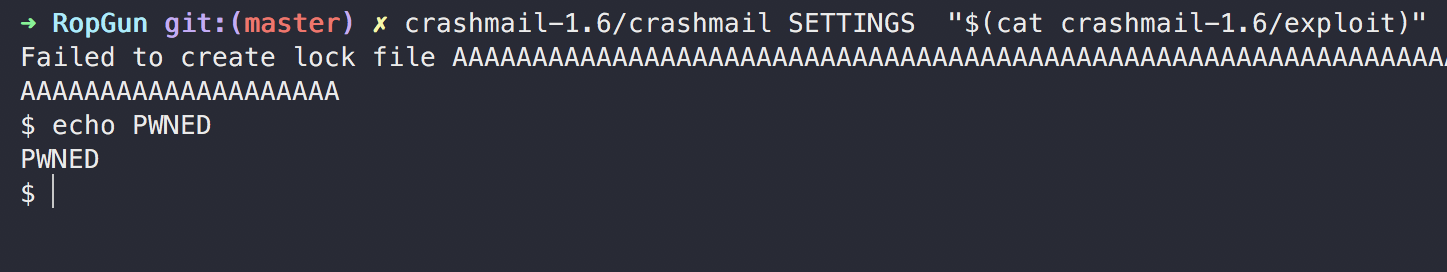
\includegraphics[width=0.9\linewidth]{exploit}
\end{center}

While monitoring the process with {\bf RopGun} clearly evidences in the log the moment of the attack:

\begin{verbatim}
$ ropgun -m crashmail-1.6/crashmail SETTINGS  "$(cat crashmail-1.6/exploit)"
\end{verbatim}

\begin{center}
  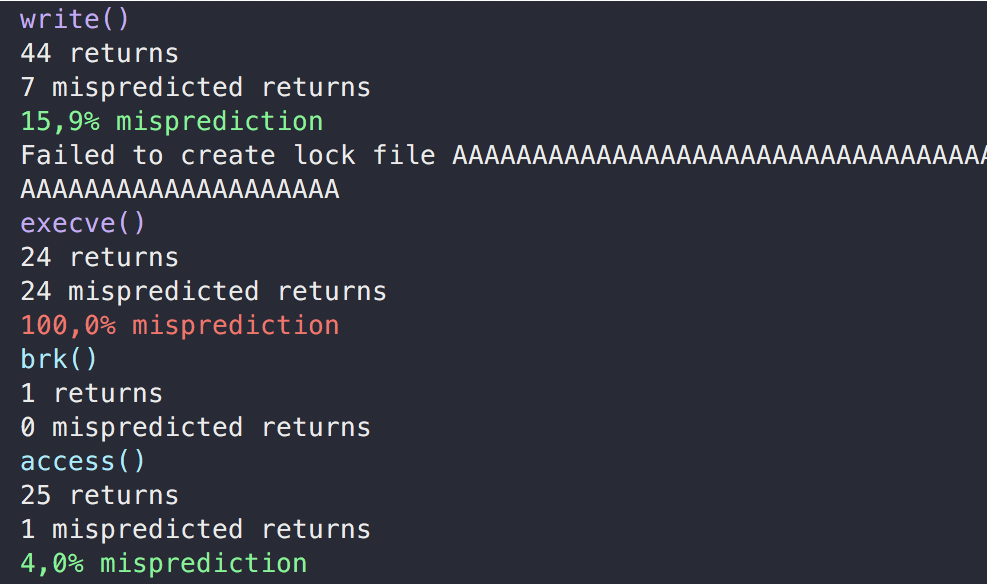
\includegraphics[width=0.9\linewidth]{monitor}
\end{center}

And our tool succeeds to block the attack while running in {\tt Killer Mode}:

\begin{center}
  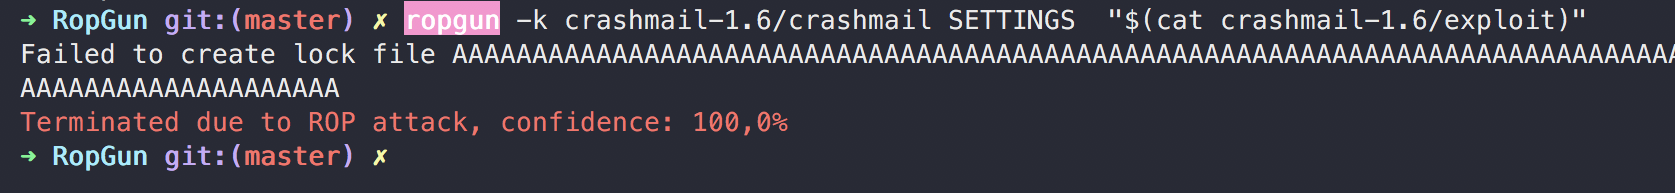
\includegraphics[width=0.9\linewidth]{killer}
\end{center}
\newpage


\begin{thebibliography}{99}
  \bibitem{kbouncer}
    Vasilias Pappas,
    kBouncer: Efficient and Transparent ROP Mitigation,
    2012.

  \bibitem{rop}
      Hovav Shacham,
      The Geometry of Innocent Flesh on the Bone: Return-into-libc without Function Calls (on the x86),
      CCS,
      2007.

  \bibitem{ret2libc}
    Nergal,
    The advanced return-into-lib(c) exploits (PaX case study),
    Phrack Magazine 58(4),
    Dec. 2001.

  \bibitem{HDROP}
    HongWei Zhou,
    HDROP: Detecting ROP Attacks Using Performance Monitoring Counters,
    ISPEC,
    2014.

  \bibitem{coop}
    Felix Schuster,
    Counterfeit Object-oriented Programming: On the Difficulty of Preventing Code Reuse Attacks in C++ Applications
    IEEE Symposium on Security and Privacy,
    2015.

  \bibitem{jop}
    Tyler Bletsch,
    Jump-Oriented Programming: A New Class of Code-Reuse Attack
    Asia CCS,
    2011

  \bibitem{crashmail}
    \path{http://ftnapps.sourceforge.net/crashmail.html}

  \bibitem{exploit}
    \path{http://www.exploit-db.com/exploits/44331/}

\end{thebibliography}

\end{document}
